% mnras_template.tex
%
% LaTeX template for creating an MNRAS paper
%
% v3.0 released 14 May 2015
% (version numbers match those of mnras.cls)
%
% Copyright (C) Royal Astronomical Society 2015
% Authors:
% Keith T. Smith (Royal Astronomical Society)

% Change log
%
% v3.0 May 2015
%    Renamed to match the new package name
%    Version number matches mnras.cls
%    A few minor tweaks to wording
% v1.0 September 2013
%    Beta testing only - never publicly released
%    First version: a simple (ish) template for creating an MNRAS paper

%%%%%%%%%%%%%%%%%%%%%%%%%%%%%%%%%%%%%%%%%%%%%%%%%%
% Basic setup. Most papers should leave these options alone.
\documentclass[a4paper,fleqn,usenatbib]{mnras}

% MNRAS is set in Times font. If you don't have this installed (most LaTeX
% installations will be fine) or prefer the old Computer Modern fonts, comment
% out the following line
\usepackage{newtxtext,newtxmath}
% Depending on your LaTeX fonts installation, you might get better results with one of these:
%\usepackage{mathptmx}
%\usepackage{txfonts}

% Use vector fonts, so it zooms properly in on-screen viewing software
% Don't change these lines unless you know what you are doing
\usepackage[T1]{fontenc}
\usepackage{ae,aecompl}


%%%%% AUTHORS - PLACE YOUR OWN PACKAGES HERE %%%%%

% Only include extra packages if you really need them. Common packages are:
\usepackage{graphicx}	% Including figure files
\usepackage{amsmath}	% Advanced maths commands
\usepackage{amssymb}	% Extra maths symbols
\usepackage{subfig}
%%%%%%%%%%%%%%%%%%%%%%%%%%%%%%%%%%%%%%%%%%%%%%%%%%

%%%%% AUTHORS - PLACE YOUR OWN COMMANDS HERE %%%%%

% Please keep new commands to a minimum, and use \newcommand not \def to avoid
% overwriting existing commands. Example:
%\newcommand{\pcm}{\,cm$^{-2}$}	% per cm-squared

%%%%%%%%%%%%%%%%%%%%%%%%%%%%%%%%%%%%%%%%%%%%%%%%%%

%%%%%%%%%%%%%%%%%%% TITLE PAGE %%%%%%%%%%%%%%%%%%%

% Title of the paper, and the short title which is used in the headers.
% Keep the title short and informative.
\title[Title]{The expected shape of the Milky Way's Dark Matter halo}

% The list of authors, and the short list which is used in the headers.
% If you need two or more lines of authors, add an extra line using \newauthor
\author[Jesus Prada,  Jaime E. Forero-Romero, Volker Springel ]{
Jesus Prada,$^{1}$\thanks{E-mail: jd.prada1760@uniandes.edu.co}
Jaime E. Forero-Romero,$^{1}$
Volker Springel$^{2}$
\\
% List of institutions
$^{1}$Departamento de F\'sica, Universidad de los Andes, Cra. 1 No.
18A-10, Edificio Ip, Bogot\', Colombia.\\
$^{2}$Heidelberg Institute for Theoretical Studies, Schloss-Wolfsbrunnenweg 35, D-69118 Heidelberg
Germany.\\
}

% These dates will be filled out by the publisher
\date{Accepted XXX. Received YYY; in original form ZZZ}

% Enter the current year, for the copyright statements etc.
\pubyear{2018}

% Don't change these lines
\begin{document}
\label{firstpage}
\pagerange{\pageref{firstpage}--\pageref{lastpage}}
\maketitle

% Abstract of the paper
\begin{abstract}
This is a simple template for authors to write new MNRAS papers.
The abstract should briefly describe the aims, methods, and main results of the paper.
It should be a single paragraph not more than 250 words (200 words for Letters).
No references should appear in the abstract.This is a simple template for authors to write new MNRAS papers.
The abstract should briefly describe the aims, methods, and main results of the paper.
It should be a single paragraph not more than 250 words (200 words for Letters).
No references should appear in the abstractThis is a simple template for authors to write new MNRAS papers.
The abstract should briefly describe the aims, methods, and main results of the paper.
It should be a single paragraph not more than 250 words (200 words for Letters).
No references should appear in the abstract
\end{abstract}

% Select between one and six entries from the list of approved keywords.
% Don't make up new ones.
\begin{keywords}
keyword1 -- keyword2 -- keyword3
\end{keywords}

%%%%%%%%%%%%%%%%%%%%%%%%%%%%%%%%%%%%%%%%%%%%%%%%%%

%%%%%%%%%%%%%%%%% BODY OF PAPER %%%%%%%%%%%%%%%%%%

\section{Introduction}

%This is a simple template for authors to write new MNRAS papers.
%See \texttt{mnras\_sample.tex} for a more complex example, and \texttt{mnras\_guide.tex}
%for a full user guide.

All papers should start with an Introduction section, which sets the work
in context, cites relevant earlier studies in the field by \citet{Others2013},
and describes the problem the authors aim to solve \citep[e.g.][]{Author2012}.\\

Introduce/ Motivation simulations, sphereical top hat collapse.\\

One of the principal predictions of the CDM model is that DM halos are ellipsoidal and very well characterized by the principal axes $a>b>c$. This is due, among other causes, to the anisotropical and clumpy accretion of matter influenced by environmental structures \citep[see?][]{environment-shape}. The general concensus in numerical simulations \citep[e.g.][]{TriaxialHalos1,TriaxialHalos2,etc} is that halos tend to be prolate with axial ratios b/a ~ \textit{number}, c/a ~ \textit{number} and small differences may arise by the use different methods in numerical recipies for the simulations and the shape-calculation methods  \citep[see][]{Allgood et al. 2006}. Some studies have gone a step further as for analyzing the dependence of shape of the DM halo on the radius and redshift \citep[e.g.][]{Shape-radius-papers, including Allgood}, generally finding that halos are rounder at the outerskirts and at lower redshift.\\

Due to the evasive nature of DM, properly constraining the shape of DM halos is a very difficult endeavour.\\

Better connector with observations of distant galaxies. Gravitational lensing and star tracers. (Talk about discrepancy with simulations, perhaps later) and state that the preference for axisymmetrical shapes may arise from the observational restrictions (projection) look for citations about this .\\

In the case of the Milky Way, where we have a three-dimensional view from the inside, there seems to be a general agreement for oblate (i.e. a=b>c) configurations at small distances around \~ <20kpc \citep[see][]{LM10,Bovy2016,Loebman,Vera-Ciro, RobOllingMerrifield,Bovy,BanerjeeChanda}, and more triaxial and prolate configurations on the outter distances \~>20kpc \citep[see][]{Vera-Ciro,LMJ09,Deg,BanerjeeChanda}. However, some studies are inclined towards prolate configurations even at the inner parts of the halo \citep[see][]{BowdenEvansWilliams,Findothers}, and although it previously seemed that a triaxial DM halo on the outerskirts would be necessary to fully explain the characterization of the Sagittarius stream \citep[see][]{LMJ09}, more recent studies put into doubt (question) this claim by reporting inconsistencies with narrow stellar streams \citet{PearsonKupperJohtnston, MoreLikeThis} or finding that the relaxation of other constraints may make this claim unnecessary (wording) \citet{IbataLewisMartin}.\\

Although observations predict more symmetric halos than DM-only simulations, this may be an effect of not taking into account the gravitational effects of baryonic matter. The collapse of baryonic matter generate denser structures than those of DM only, whose potential may affect the kinematics that give shape to DM halos by making them more axisymmetrical. Regarding the specifics of this rounding effect and stability, there is much to be known as the simulation of baryonic dynamics in the whole cosmological context to galactic-scale resolution is not a trivial task and is usually subject to simplifications to analyze extreme cases as boundary constrains. Simple study the adiabatical growth of a disk potential in DM halos of different triaxiality and in different orientations \cite{Debattista-Moore,Debattista-Roskar}. While these studies are elucidating about dynamical aspects that may play important roles in the shape rounding, they neglect some important galactic properties that may also contribute to this rounding that can be only analyzed with more sophisticated hydrodynamical simulations with restricted models of feedback \cite{Abadi-Navarro,Bryan-Kay}. In this way, it can be demonstrated that the galaxy formation efficiency \cite{Abadi} and the history of formation may also determine the extent of this rounding.\\

In this work, we analyze the Auriga simulations wich etc, where we can analyze the effect of dynamical properties of baryons together with galactic features, that are involved in the shaping of the DM halo shape of realistic MW-like galaxies.

\section{Numerical Simulations}
In this work we use the results of the state-of-the art Auriga simulations \cite{auriga}. It selected a set of 30 isolated halos from the Evolution and Assembly of GaLaxies and their Environments (EAGLE) project \cite{Eagle}. Each halo was identified with the algorithm "Friend of Friends" (FOF) \cite{Davis_et_al._1985}, which recursively links particles if they are closer than some threshold distance referred as linking length. EAGLE follows the evolution of fixed-mass particles of $m_{\text{DM}} = 1.15\cdot 10^7\text{M}_{\odot}$ from $z=127$ to $z=0$, adopting the $\Lambda$CDM model from the \cite[Planck Collaboration et al. (2014)]{Planck_Collaboration_2014}, which is characterized by $\Omega_\Lambda=0.693$, $\Omega_\text{m}=0.307$, $\Omega_\text{b}=0.048$ \& $\text{H}_0=67.77\text{kms} ^{-1}\text{Mpc}^{-1}$. 

These halos were randomly selected from a sample of the most isolated quartile of halos whose virial mass $M_{200}$ varied between $10^{12}M_\odot$ and $2\cdot 10^{12}M_\odot$. \textbf{\tiny This mass is defined as the mass enclosed within the virial radius $R_{200}$ at which the density becomes 200 times the critical density of the universe. \huge FOOTNOTE \normalsize}. These halos were re-simulated with the (AREPOOO HERE) by increasing the mass resolution of the particles belonging to them and diminishing the resolution of the rest of the particles.\\

Various versions of each halo were modelled with different degrees of realism. All 30 halos were simulated within a level-4-degree of resolution defined for Aquarius simulations corresponding to $\tilde 3\cdot 10^6$ high resolution particles of $\tilde 2.5 \cdot 10^5 M_\odot$. The principal details of each of these halos are consigned on the table \ref{tab:level4}. From these halos, 6 of them where re-simulated at level 3 (higher) resolution taking into account a spatial factor of 2 in each dimension. For more information about level 3 halos, their details are printed on table \ref{tab:level3}. Furthermore, fore each halo in each level of resolution there are two versions of the simulation. One of tracks the evolution of DM-only particles while the remaining one evolves DM and baryions with magneto-hydrodynamical (MHD) physics, including DM.\\


\section{Determining the halo shape}

%\subsection{The solid ellipsoid method}

There is no trivial way to calculate the DM halo shape at a determined radius due to the discretization of particles. For practical effects, observational models focus on the shape of the DM isopotential \cite{isopotential} or isodensity \cite{isodensity} contours. In cosmological simulations, it is preferred to work with the isodensity contours which is directly calculated from particle positions. However, these density contours are not smooth and are very sensitive to the presence of small satelites \cite{Springel Isodensity}. For this reason we determine the shape taking into account volume-enclosed particles, rather than shell-enclosed. While this approach allows the cumulative influence of outter shells on the outter shapes, it has been demonstrated for DM-only simulations that this effect becomes important only for big radii \cite{vera-Ciro aquarius}.  We therefore follow the method of \cite[Allgood et al. 2006]{Allgood_et_al._2006} that consits in the use of the reduced inertia tensor,   \\

\begin{equation}
I_{ij} = \sum_k \frac{x_k^{(i)}x_k^{(j)}}{d^2_k},
\label{eq:inertia}
\end{equation}

with components weighted by the k-th particle distance $d^2=x^2+y^2+z^2$.\\

The diagonalization of this tensor yields the principal axes of the structure as well as the eigen-quantities which are proportional to the squared principal axes $a>b>c$. We start our calculations taking into account particles within a sphere of radius $R$ and then recharacterize the triaxial parameters by taking into account particles within an ellipsoid of semi-axes $r,r/q,r/s$ and weighted distance $d^2=x^2+(y/q)^2+(z/s)^2$, where ere $q = b/a$ and $s=c/a$ are the previously calculated axial ratios. We repeat this process until the average deviation of semi-axes is less than $10^{-6}$.\\

\section{Results}
For convergence reasons and seeking to make our results observation-comparable, we restrict the sampling of the ellipsoidal parameters to radii between $1/16 R_{vir} and 2R_{vir}$ of the virial radius $R_{500}$, defined as the (DEFINITION OF VIRIAL RADIUS). All our results make use of this reference radius unless strictly stated otherwise.\\ 

\subsection{The radial tendency of axial ratios}
To have a more complete picture about the effect of baryons on the DM halo shape, we begin by verifying/understanding the radial evolution (dependence?) of the shape. In the case of DM-only simulations, it is expected that halos get monotonically rounder at larger radii due to the gravitational effect of inner shells \citep{Vera-Ciro et al. 2012}. A graphic example of this rounding can be checked on figure \ref{fig:DM_MHD}, where we plot the a projection of a DM-only halo aligned with the calculated minor axis at two different radius together with the estimated projected ellipsoidal. Formally, this effect is reflected in the axial ratios $b/a,c/a$, which tend to unity on the outerskirts of the halo. As a representative sample of this relations, we show on figure \ref{fig:DM relation} the evolution of the axial ratios $b/a,c/a$ and the triaxiality parameter $T=\frac{a^2-b^2}{a^2-c^2}$ in a wide range of radii.\\

In general, we find that DM-only halos are shaped with parameters in table \ref{table:DM table}. To show this relation is real and not a result of strong peculiarities of particular DM halos, we resume the results of the 30 auriga simulations on the figure \ref{fig: triaxial plane} where each shape represents a point in the triaxiality plane $c/a Vs b/a$. Check Vera-ciro onthis.\\

 

\begin{figure}
  \centering
  \subfloat[halo 27 DM shape at small radius]{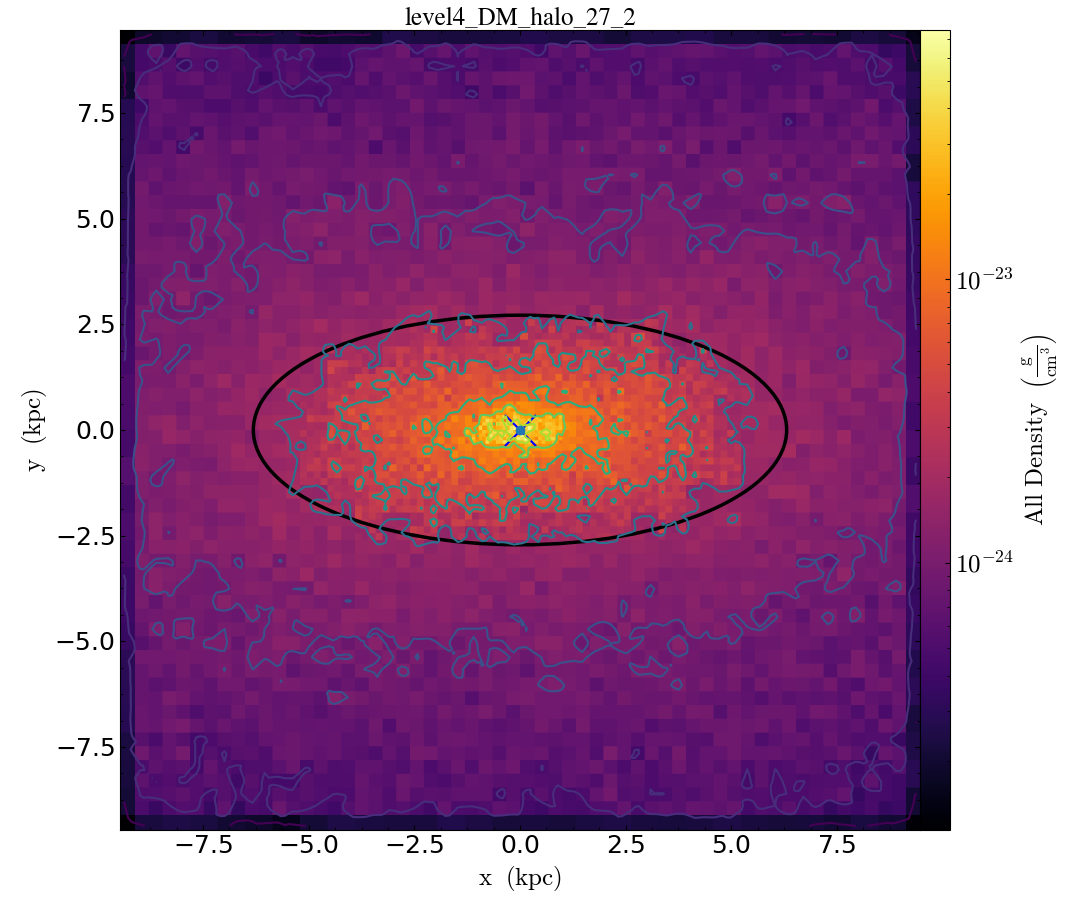
\includegraphics[width=0.5\columnwidth]{./pics/MHD_Vs_DM/level4_DM_halo_27_inner.png}}
  \hfill
  \subfloat[halo 27 DM shape at big radius]{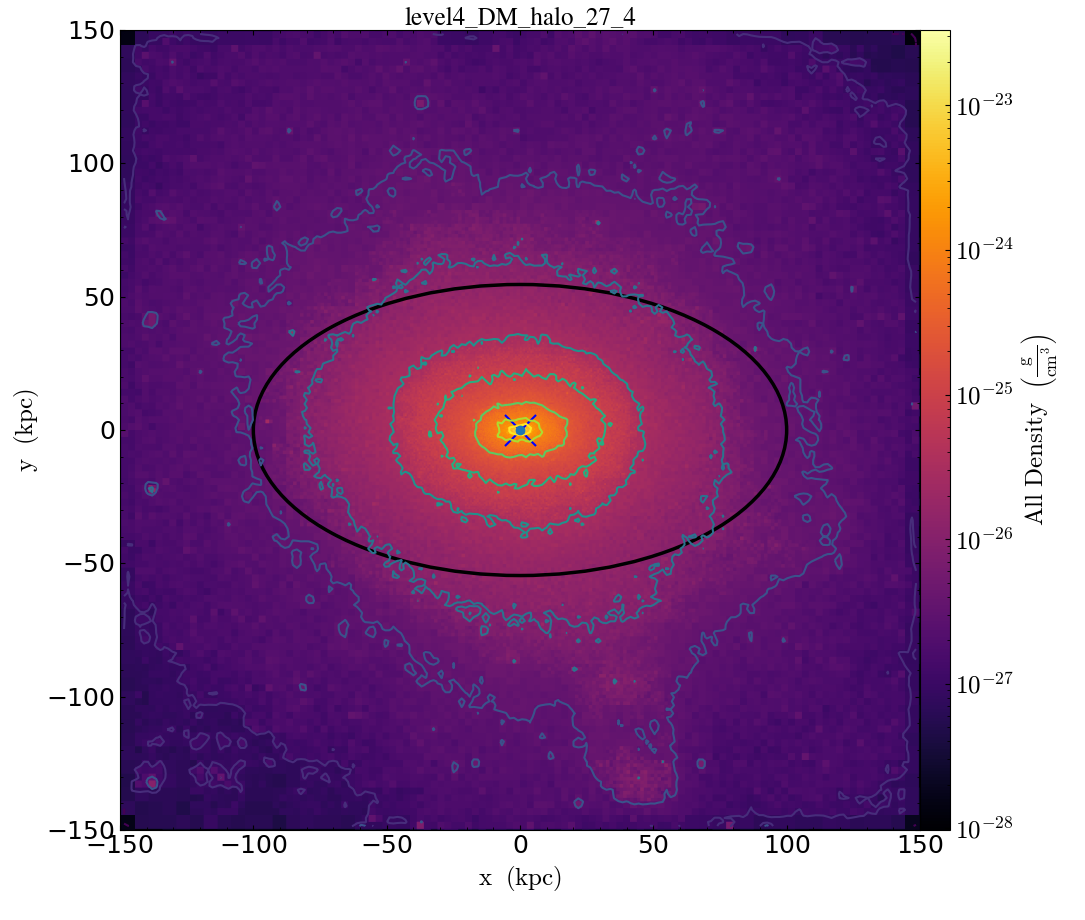
\includegraphics[width=0.5\columnwidth]{./pics/MHD_Vs_DM/level4_DM_halo_27_outter.png}}
  \hfill
  \caption{DM density for inner (outer) parts of the halo 27 on the left (right) part. The horizontal (vertical) axes are aligned to the major (medium) axes. (optimaze space and description) }
  \label{fig:slices}
\end{figure}

\begin{table}
\setlength{\tabcolsep}{3pt}
\begin{tabular}{l|cccccc}
 &$R_{1/16}$& $R_{1/8}$& $R_{1/4}$& $R_{1/2}$& $R_1$ & $R_2$\\
\hline \hline
$\bar{q}$&$0.55^{+0.07}_{-0.07}$&$0.57^{+0.09}_{-0.08}$&$0.61^{+0.15}_{-0.08}$&$0.65^{+0.18}_{-0.10}$&$0.70^{+0.13}_{-0.10}$&$0.75^{+0.10}_{-0.10}$ \\ [0.1cm]
$\bar{s}$&$0.42^{+0.12}_{-0.03}$&$0.45^{+0.11}_{-0.04}$&$0.49^{+0.09}_{-0.05}$&$0.52^{+0.10}_{-0.05}$&$0.56^{+0.10}_{-0.05}$&$0.59^{+0.11}_{-0.06}$ \\ [0.1cm]
$\bar{T}$&$0.89^{+0.03}_{-0.08}$&$0.88^{+0.04}_{-0.12}$&$0.84^{+0.08}_{-0.23}$&$0.81^{+0.08}_{-0.29}$&$0.75^{+0.14}_{-0.25}$&$0.71^{+0.16}_{-0.19}$ \\ [0.1cm]

\hline
\end{tabular}
\caption{Median values of axial ratios $q,s$ and triaxiality parameter $T$ for DM halos in DM-only simulations at different radii (columns). }
\label{tabe:DM table}
\end{table}

Concerning MHD halos, the expected tendency is not clear. Some studies claim that the DM halo must be oblate, at least in the vicinities of the disk, to ensure its stability. However, not much is said about its dependence with radius as these studies focus rather on the effects of baryons on the dynamics of the halo. Taking a look at some representative graphics similar to those presented before, \ref{fig:,fig:}, some things are noticeable: first, the halo is almost perfectly oblate around $\approx 10-30$Kpc and second: its axial ratios start decreasing very slowly after $50$ and below $10Kpc$. Overall, our results are sumarized on table \ref{MHD table}, where we included some extra measurement at twice the size of the gas disk HalfRad.\\

\begin{table}
\setlength{\tabcolsep}{3pt}
\begin{tabular}{l|ccccccc}
 &$R_{1/16}$& $R_{1/8}$& $R_{1/4}$& $R_{1/2}$& $R_1$ & $R_2$& $R_{Disk}$\\
\hline \hline
$\bar{q}$&$0.93^{+0.04}_{-0.04}$&$0.95^{+0.03}_{-0.03}$&$0.95^{+0.02}_{-0.05}$&$0.93^{+0.04}_{-0.06}$&$0.93^{+0.04}_{-0.10}$&$0.92^{+0.03}_{-0.09}$&$0.94^{+0.03}_{-0.09}$ \\[0.1cm]
$\bar{s}$&$0.73^{+0.05}_{-0.09}$&$0.73^{+0.07}_{-0.10}$&$0.73^{+0.08}_{-0.10}$&$0.73^{+0.09}_{-0.08}$&$0.75^{+0.07}_{-0.11}$&$0.74^{+0.07}_{-0.10}$&$0.71^{+0.11}_{-0.06}$ \\[0.1cm]
$\bar{T}$&$0.31^{+0.15}_{-0.22}$&$0.20^{+0.24}_{-0.12}$&$0.24^{+0.20}_{-0.12}$&$0.30^{+0.26}_{-0.16}$&$0.36^{+0.23}_{-0.23}$&$0.39^{+0.26}_{-0.13}$&$0.24^{+0.37}_{-0.10}$ \\[0.1cm]
\hline
\end{tabular}
\caption{Median values of axial ratios $q,s$ and triaxiality parameter $T$ for DM halos in MHD simulations at different radii (columns). }
\label{tabe:MHD table}
\end{table}

Talk about source of triaxiality at the inner parts of the halos (bar?). This source of triaxiality at the inner parts explains why the axial ratios are $\approx 0.95$ and not exactly $1$. We should also discuss that the decrease in the axial ratios for bigger radii may be actually bigger/steeper but it is dimmed by the contribution of inner parts.\\

If we compare with obervational values, we must at least take isodensity contours (). We present this comparison  at two different radii for MHD simulations on figure \ref{fig:}. \\

Little discussion: Are our results congruent with observations? at which radii, does the DM halo shape vary that much?.\\

\begin{figure}
  \centering
 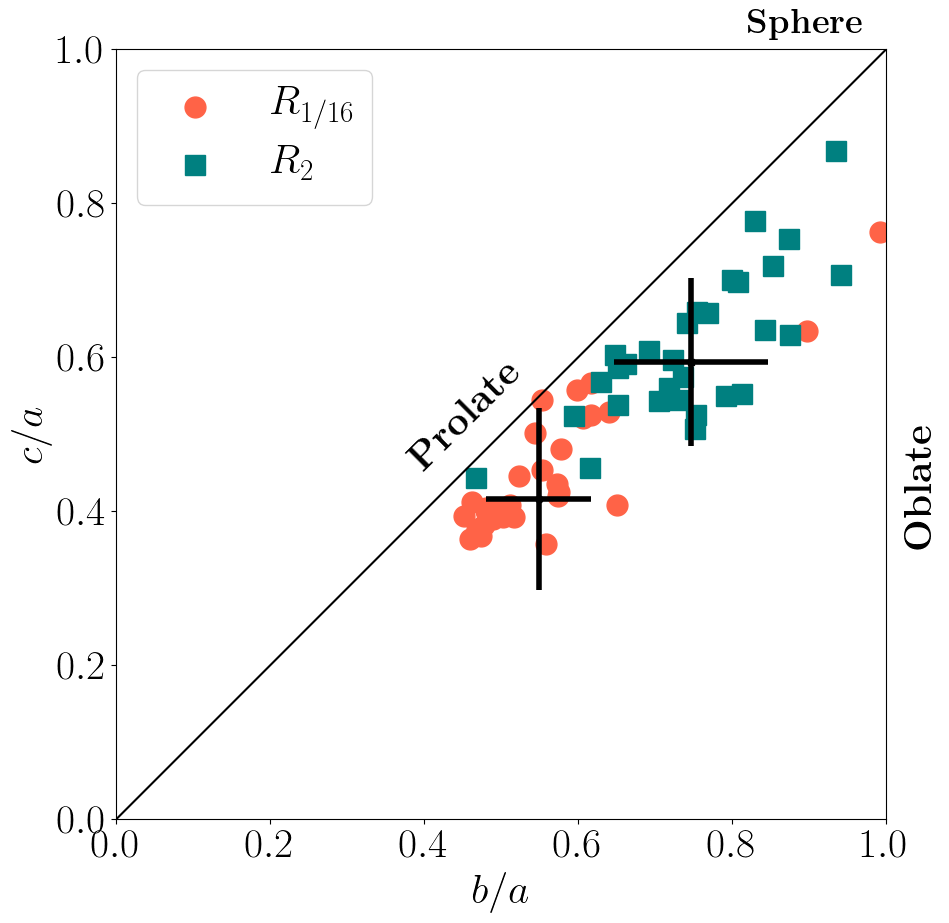
\includegraphics[width=0.9\columnwidth]{./pics/Triaxial_Plane/Triax_DM.png}
  
  \hfill
  \caption{Shape of each halo on the plane $c/a$ Vs $b/a$. Errorbar shows median and errors for each sampled radii. }
  \label{fig:Triax_DM}
\end{figure}

\subsection{The rounding effect of baryons}

\begin{figure}
\centering
{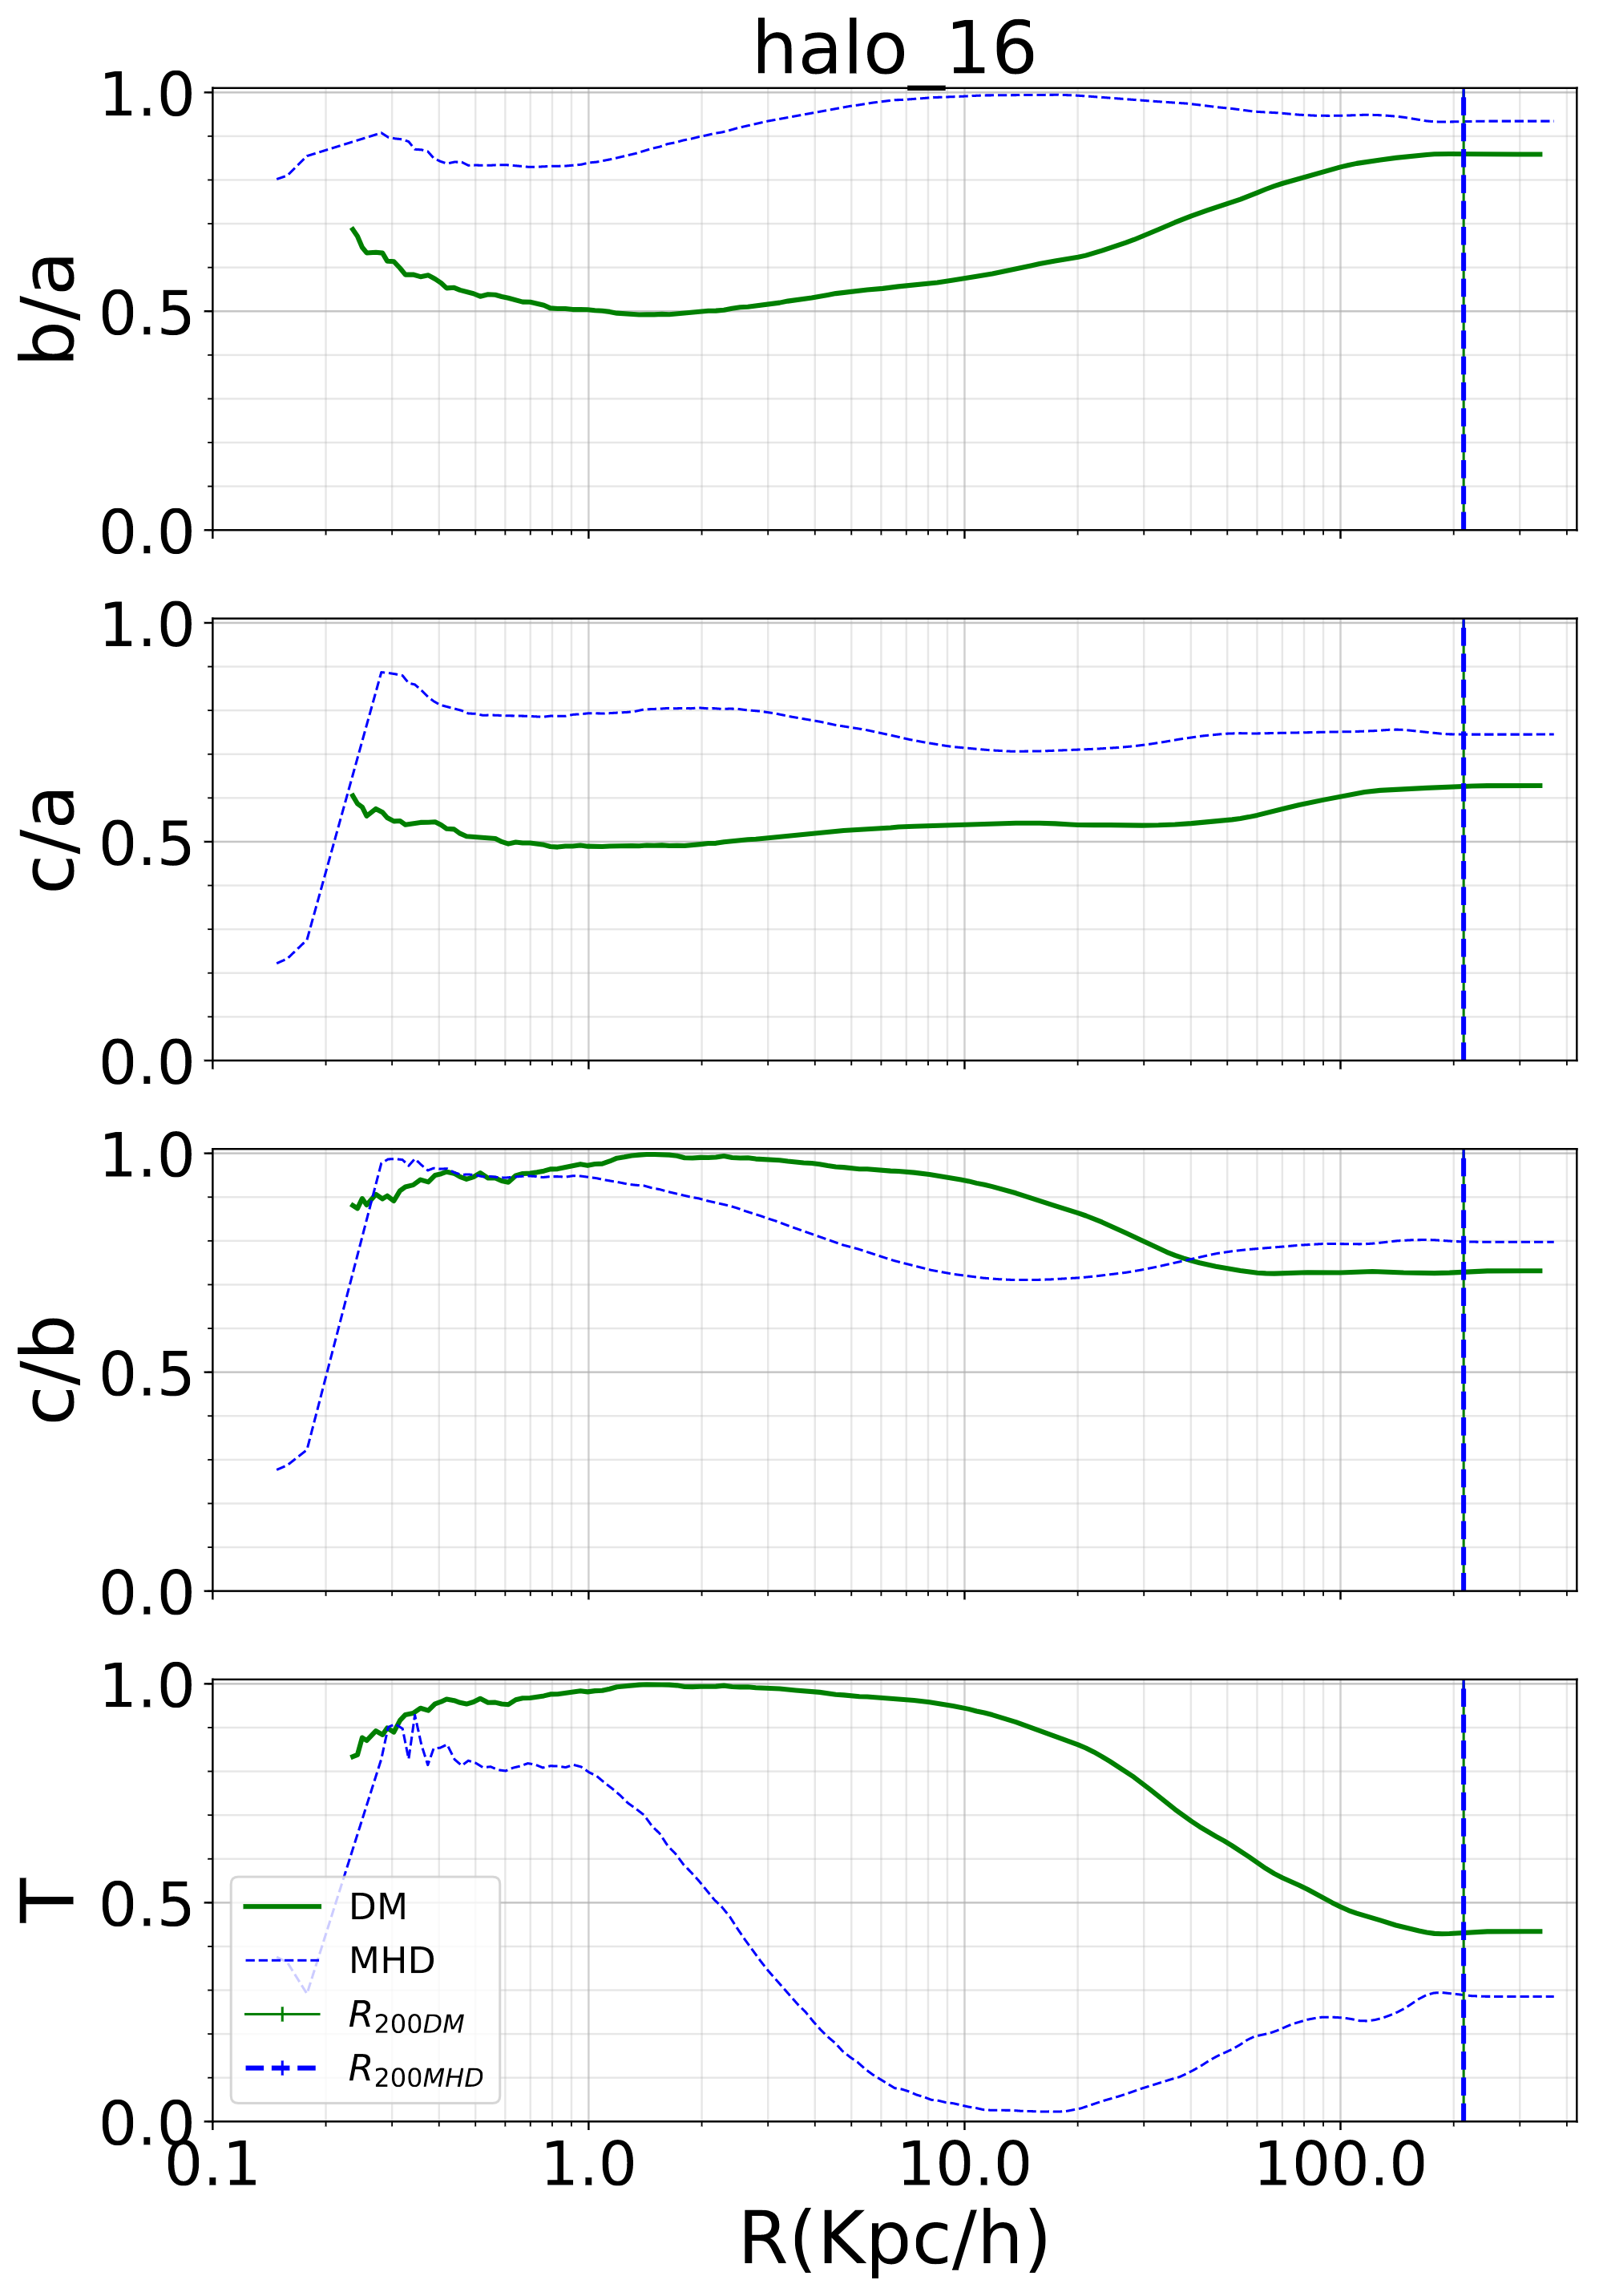
\includegraphics[width=0.8\columnwidth]{./pics/halo16.png}}
\caption{Radial profile for axial ratios and the triaxiality parameter $T=\frac{1-b/a}{1-c/a}$ from halo 16 and halo 16. These halos have a clear radial tendence towards sphericity (for smaller radii until $\approx 3$Kpc), which can be confirmed with the triaxiality parameter. (Merged Column)}
\label{fig:DM_MHD}
\end{figure} 

It is expected etc. show an example? or compare statistics? 

\begin{figure}
  \centering
  \subfloat[Level4 MHD Vs DM at inner regions]{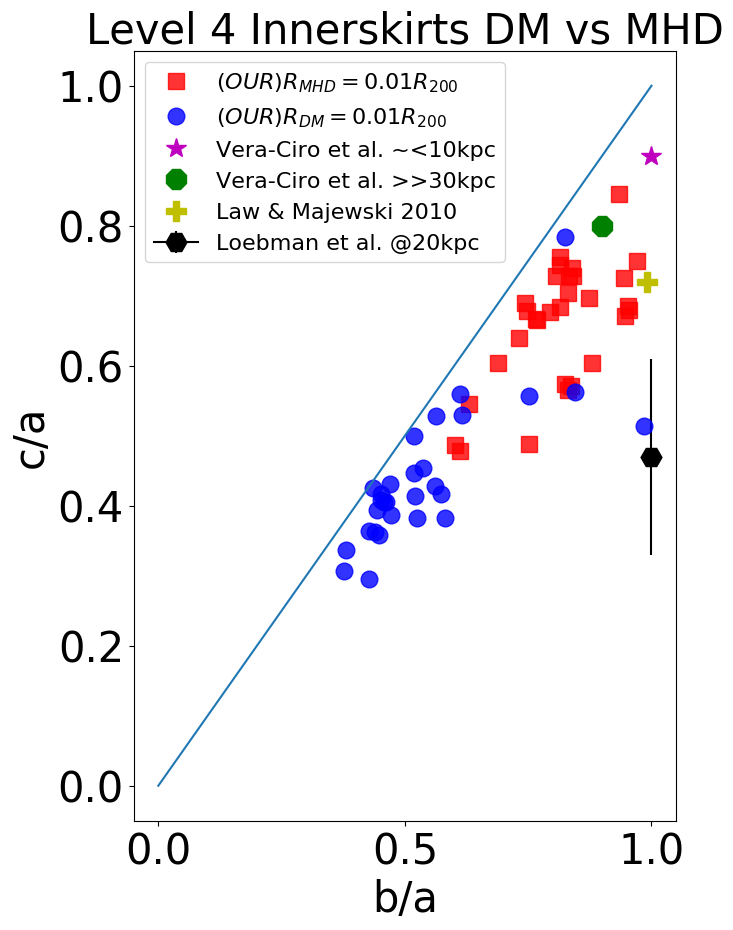
\includegraphics[width=0.5\columnwidth]{./pics/Triaxial_Plane/Triaxiality_Inner_lvl4.png}}
  \hfill
  \subfloat[Level4 MHD Vs DM at outer regions]{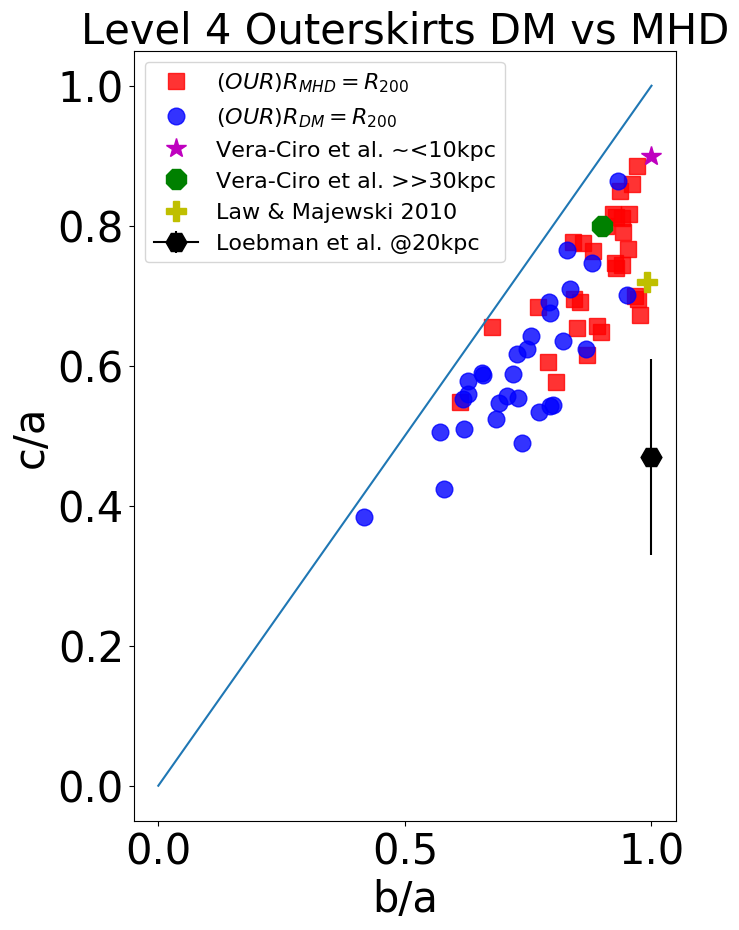
\includegraphics[width=0.5\columnwidth]{./pics/Triaxial_Plane/Triaxiality_Outter_lvl4.png}}
  \hfill
  \caption{Axial ratios as shown on $c/a$ Vs $b/a$. Each dot represents a halo shape at some radius. Some observational constraints are plotted alongside our results. Here, dots are clustered, proving the general tendence of halos to get rounder on the outer parts.(Optimize space. caption replaces title.  Present constraints representation of density)}
  \label{fig:Triaxiality_Inner_Outer}
\end{figure}

\begin{figure}
	% To include a figure from a file named example.*
	% Allowable file formats are eps or ps if compiling using latex
	% or pdf, png, jpg if compiling using pdflatex
	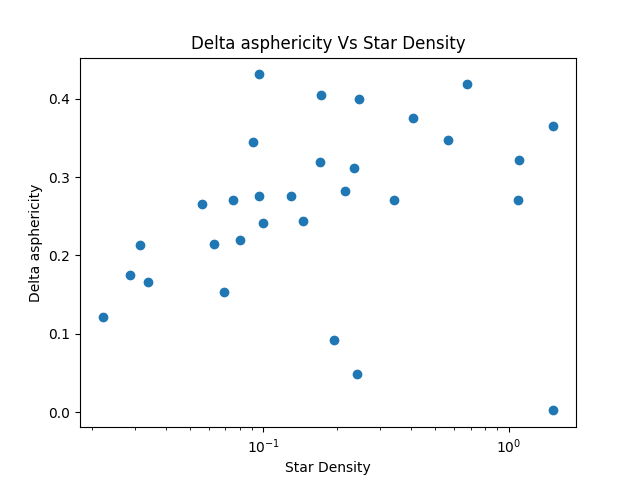
\includegraphics[width=\columnwidth]{./pics/Delta asphericity Vs Star Density.png}
    \caption{Difference in asphericities between MHD and DM shapes Vs Star Density of the simulation.}
    \label{fig:Star_Density_effect}
\end{figure}

\subsection{The historical shape}
One of the principal motivations to study the radial dependence of the DM halo shape is that it may encode some clues about its formation history. We have already shown that DM-only halos seem to exhibit a steady and monotonous growth in its axial ratios when sampled at bigger radii. One similar effect can be found if we sample the shape at the virial radius, this time at varying redshift. It is easy to see that the axial ratios increase with decreasing redshift, which is expected by the continuous influence of the gravitational potential \cite{VeraCiro}. \\   


Interestingly, these two parametic plots i.e. $(b/a,c/a)(z=0,r)$ and $(b/a,c/a)(z,r=R_{vir})$ are very correlated for DM only halos \ref{fig:redshift correlation}. This means that, for DM-only halos, one can approximate its shape at the virial radius at higher redshift by simply sampling its current shape at a smaller radius. This relationship relies strongly on the steady and monotonous tendency of DM halos towards sphericity for bigger radii and smaller redshift.\\

\begin{figure}
  \centering
  \subfloat[halo 16 DM]{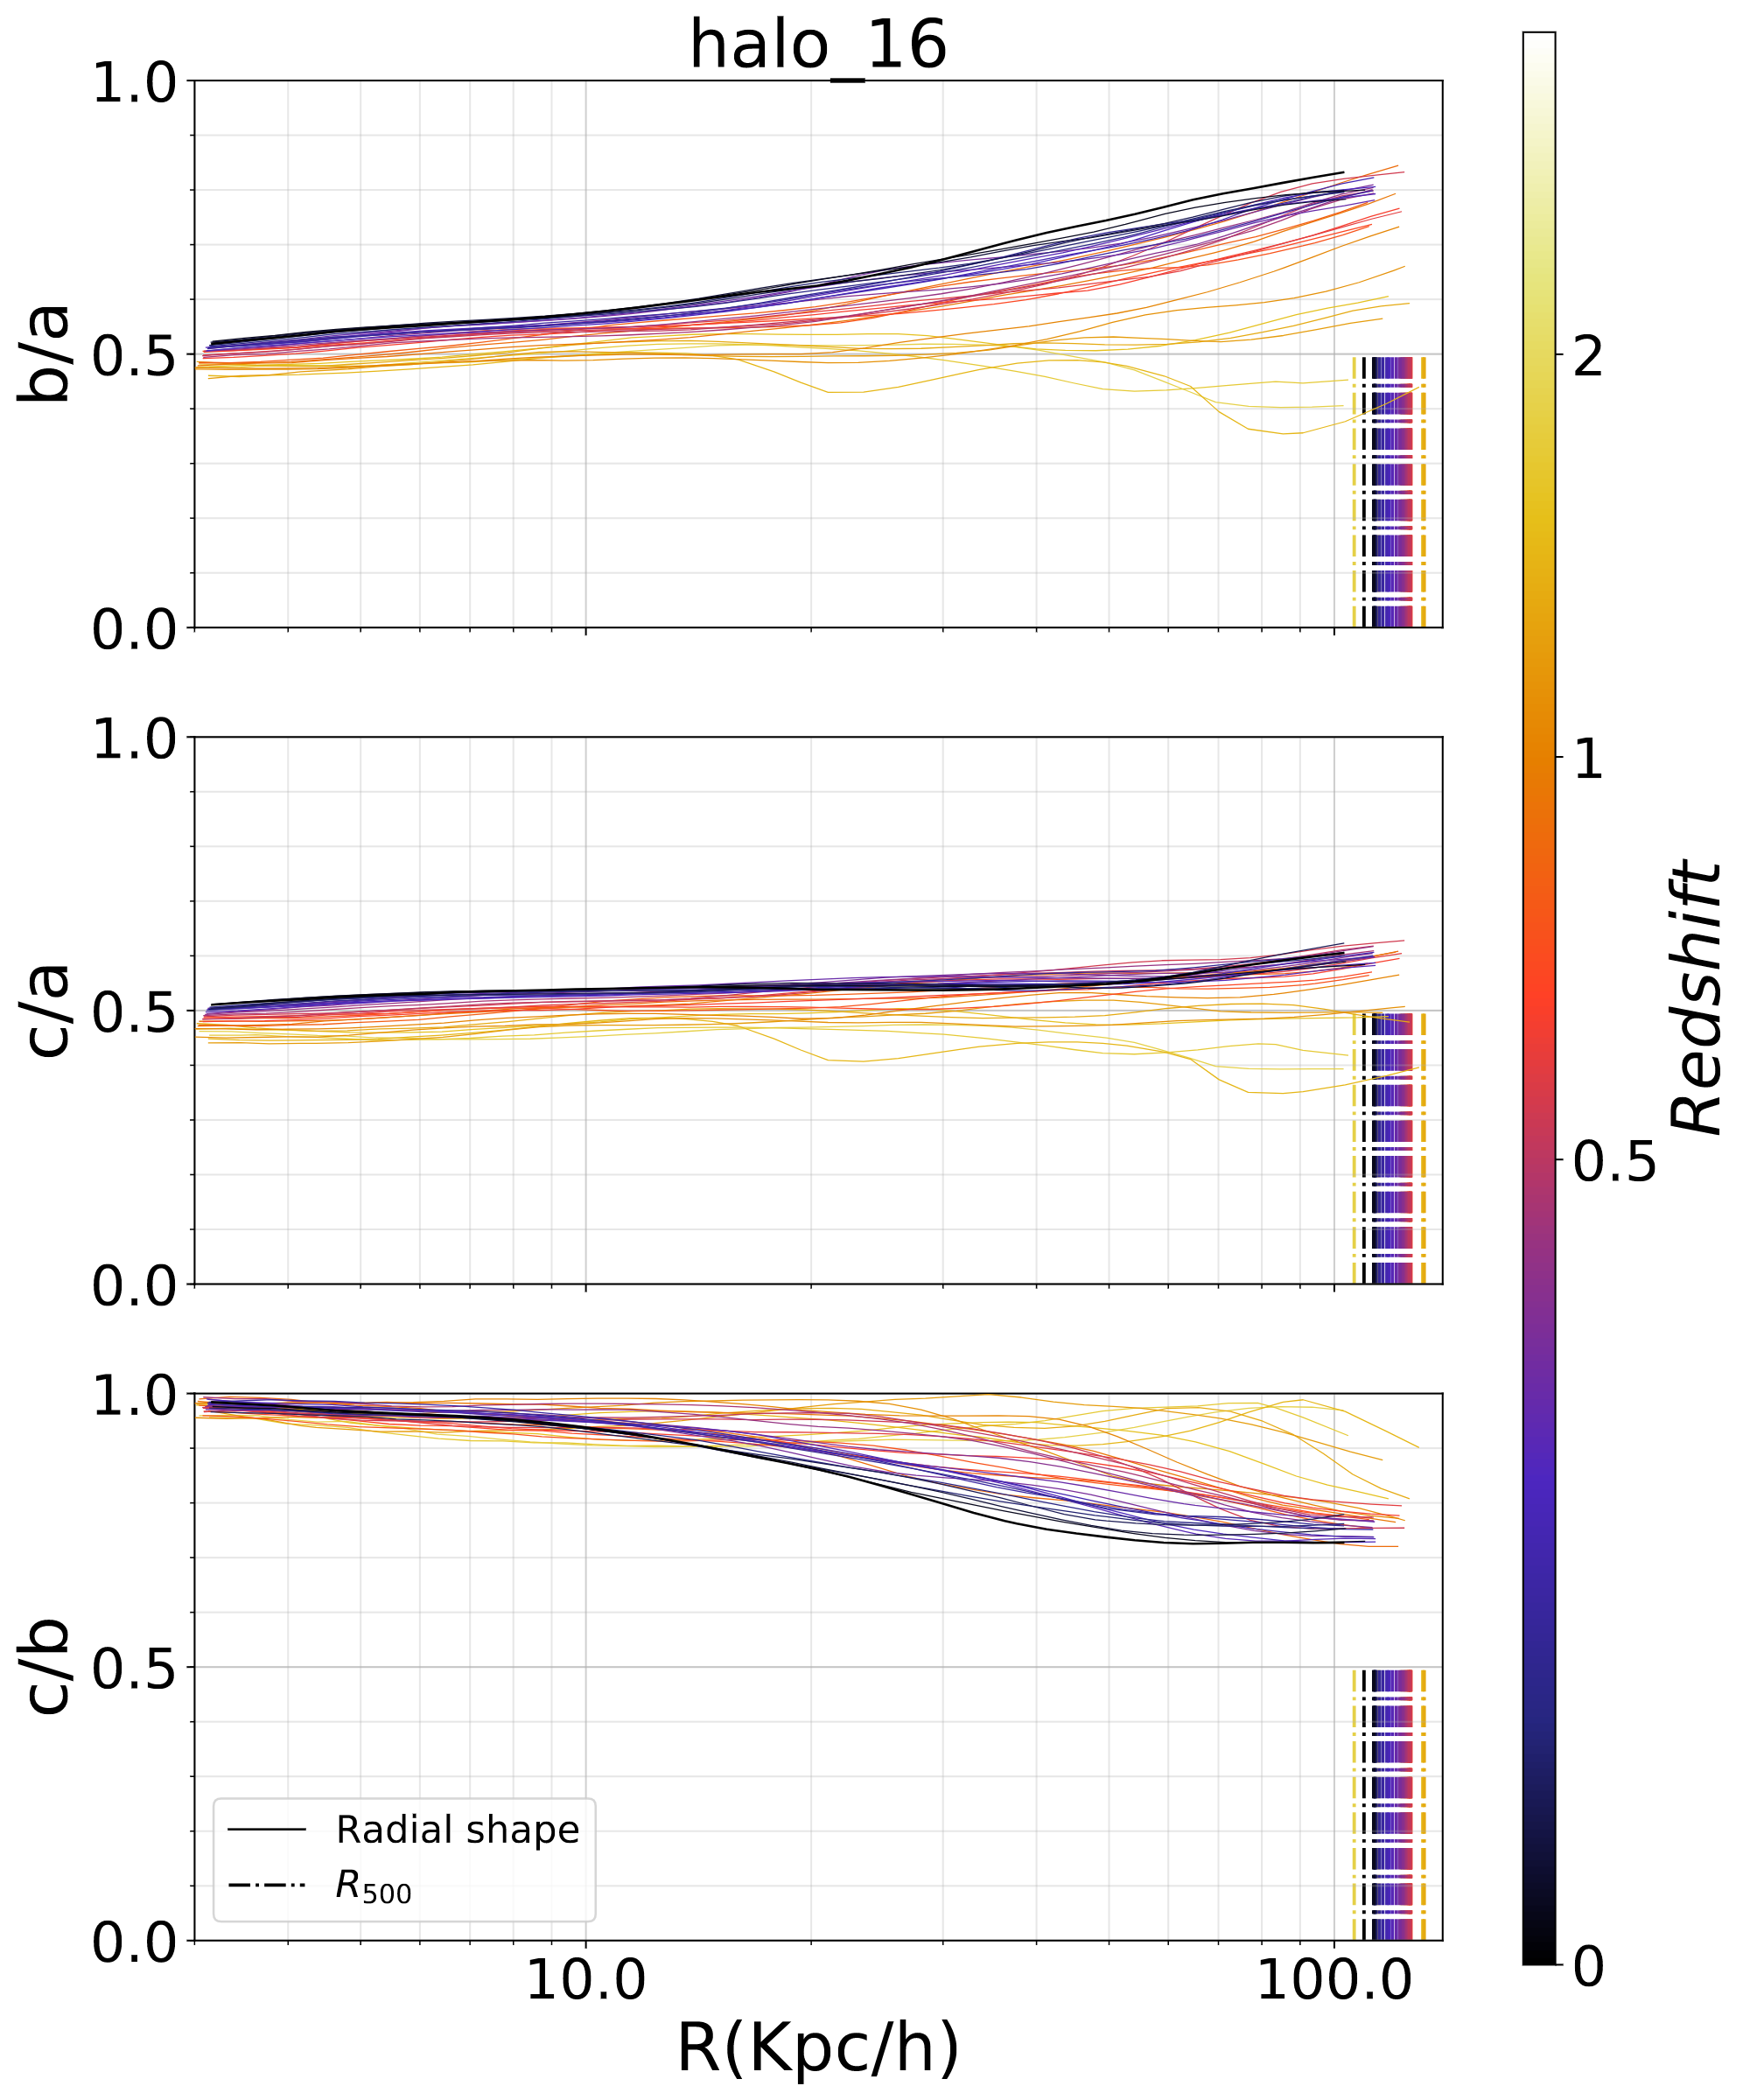
\includegraphics[width=0.5\columnwidth]{./pics/Redshift/halo_16_level3_DM_Z.png}}
  \hfill
  \subfloat[halo 16 MHD]{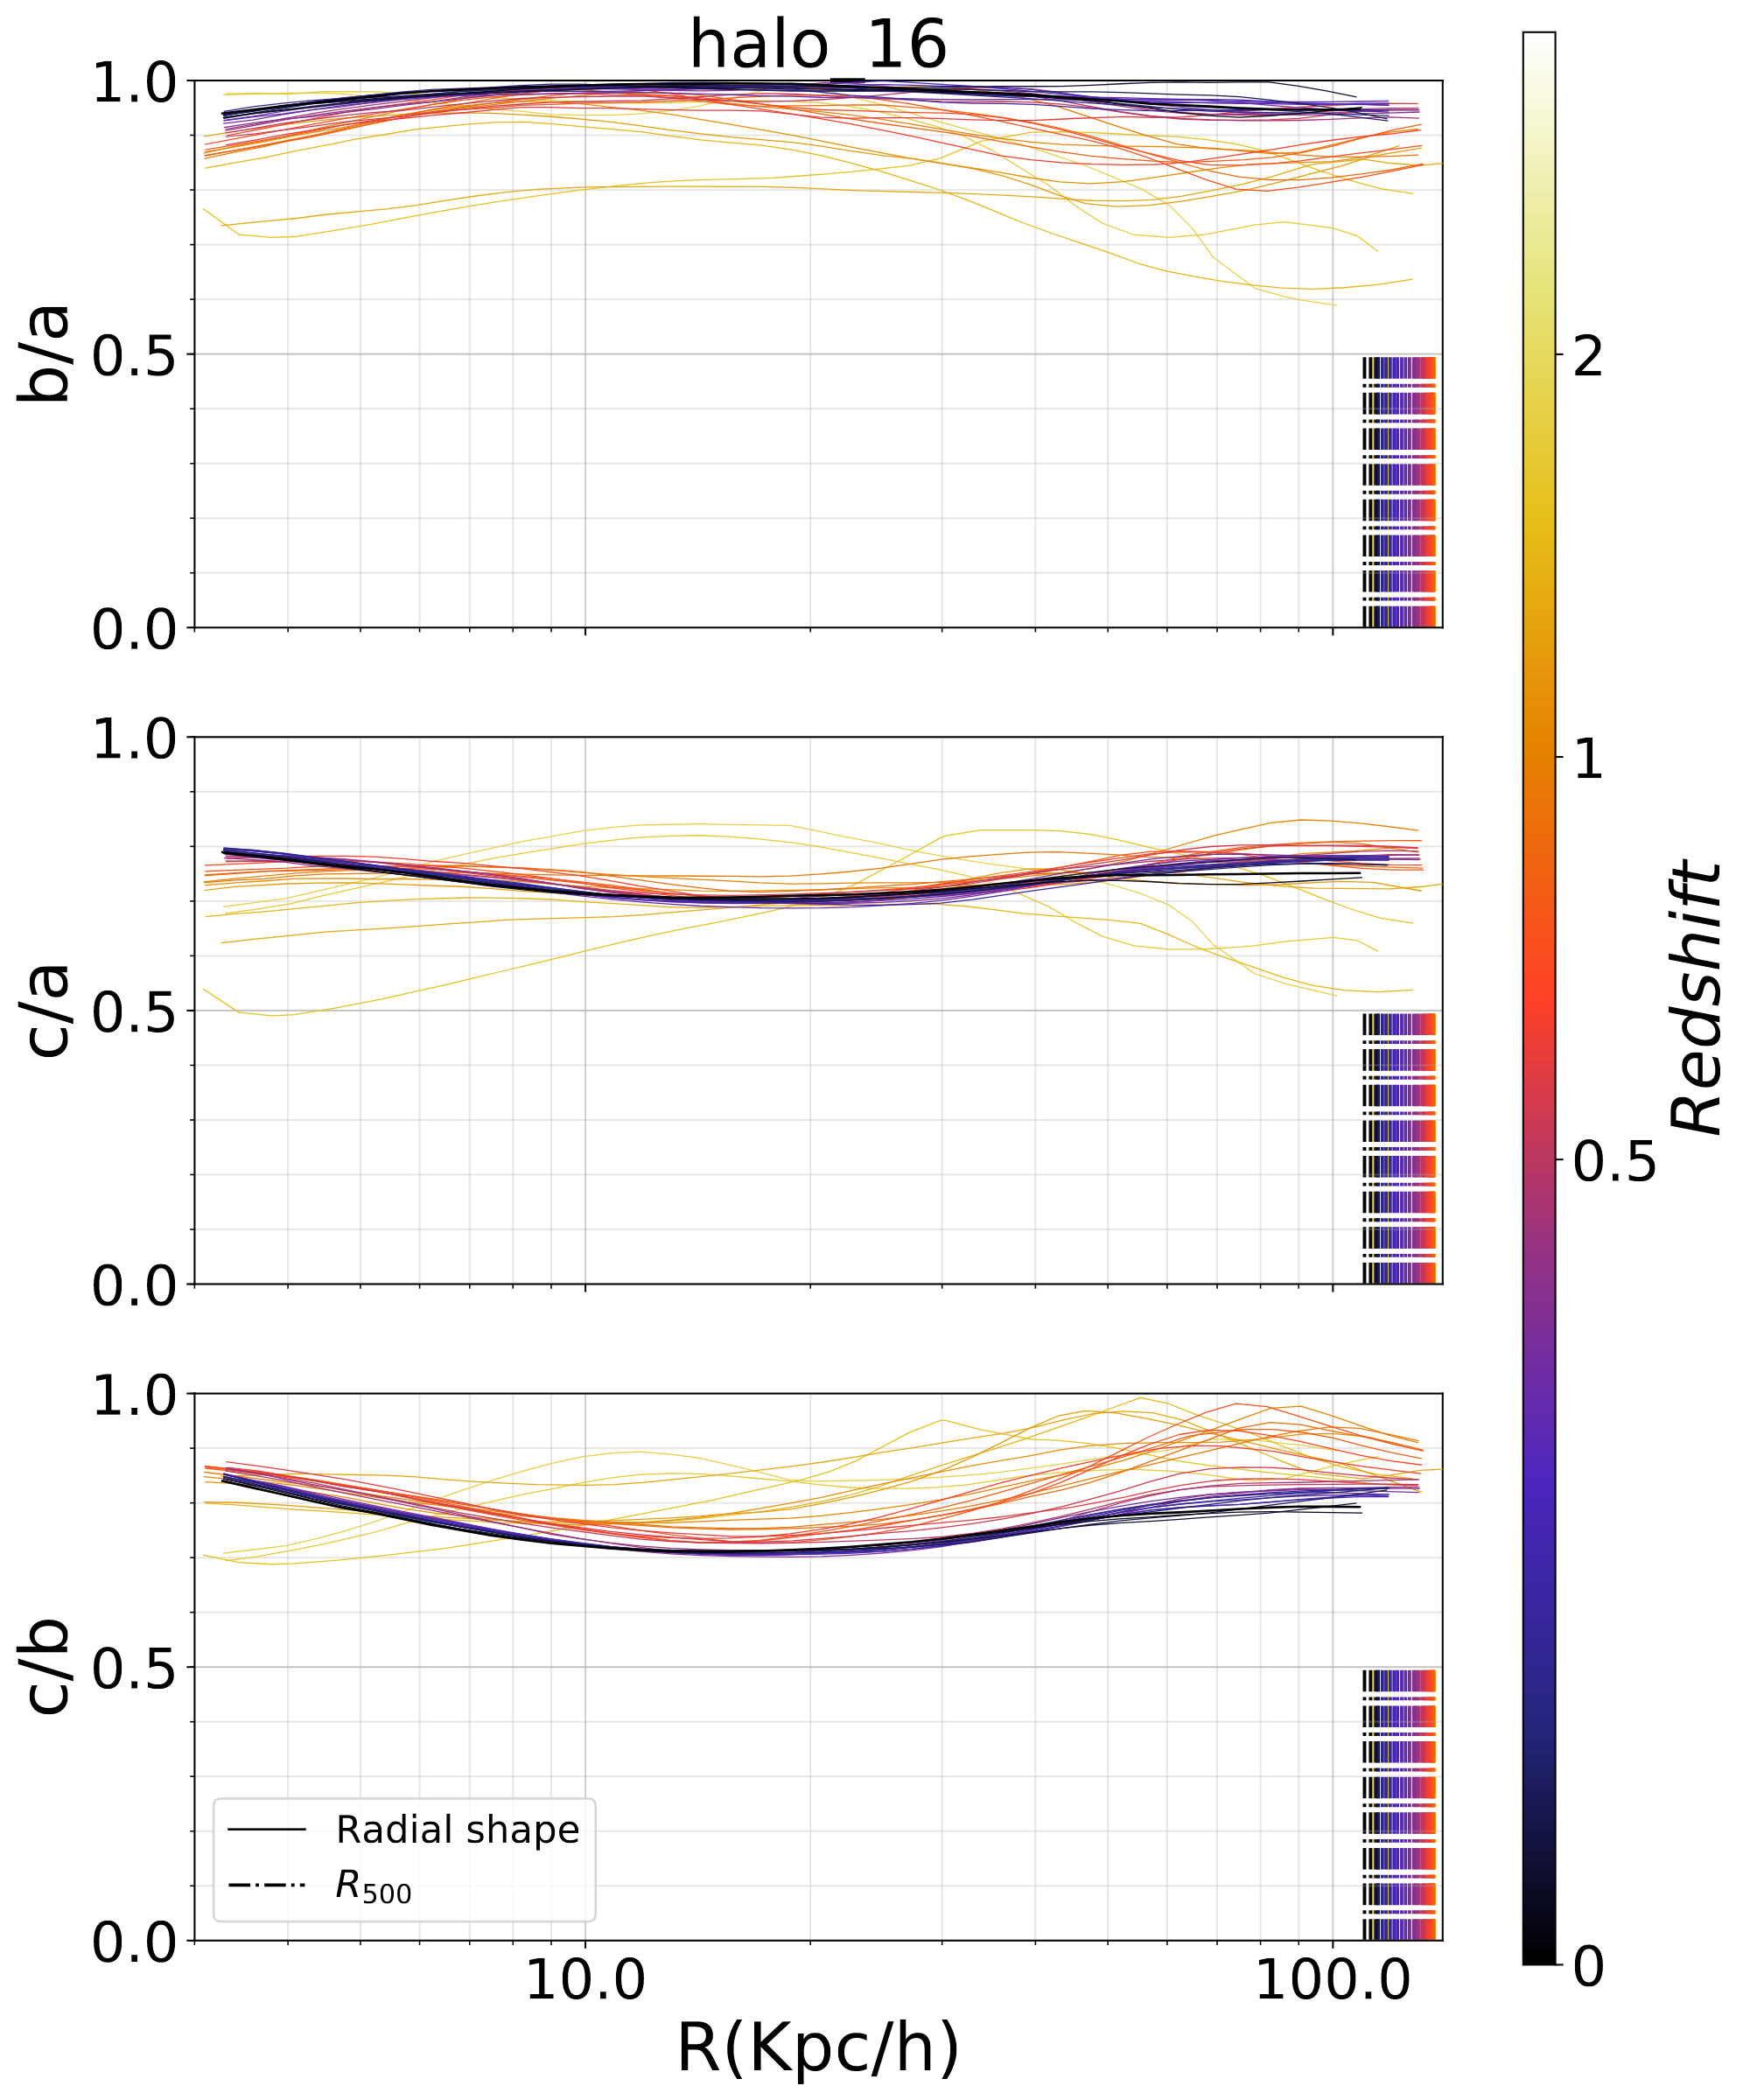
\includegraphics[width=0.5\columnwidth]{./pics/Redshift/halo_16_level3_MHD_Z.png}}
  \caption{Radial profile (comoving) of axial ratios for halo 16 in terms of redshift (color). This halo maintains its shape until $z\approx 1$ obviating the systematic rounding effect in time from asymmetric potentials. }
  \label{fig:RedshiftGood}
\end{figure}

MHD halos, on the other hand, do not exhibit tendency towards sphericity with bigger radii, but they do get sistematically rounder at lower redshift \ref{fig:MHD profile radius and redshift}. This effectively vanishes this correlation as seen from a DM halo \ref{fig:MHD Z Triax}.\\

Discuss if this correlation may be recovered if compared for example at Disk radius in stead of virial radius.\\


\subsection{The orientation of the principa axes}
This is an important result of our study. We study the radial evolution of the principal axes, compared also to the angular momentum vector from the disk. We found that while the angular momentum tend to be aligned with the minor axis of the ellipsoid, this may not be the case all times. When there is an alignment it is usually within 20 degrees (get a histogram of this. and an evolution of this histogram with time). When there is not an alignment, then there is no simple way to determine towards which axis it is oriented. Furthermore, the principal axes alignment usually change with radius (rotation, swap, verify). This ask for relaxation on the strong constrains on the MW DM halo models. 


\begin{figure}
  \centering
  \subfloat[Aligned Axes]{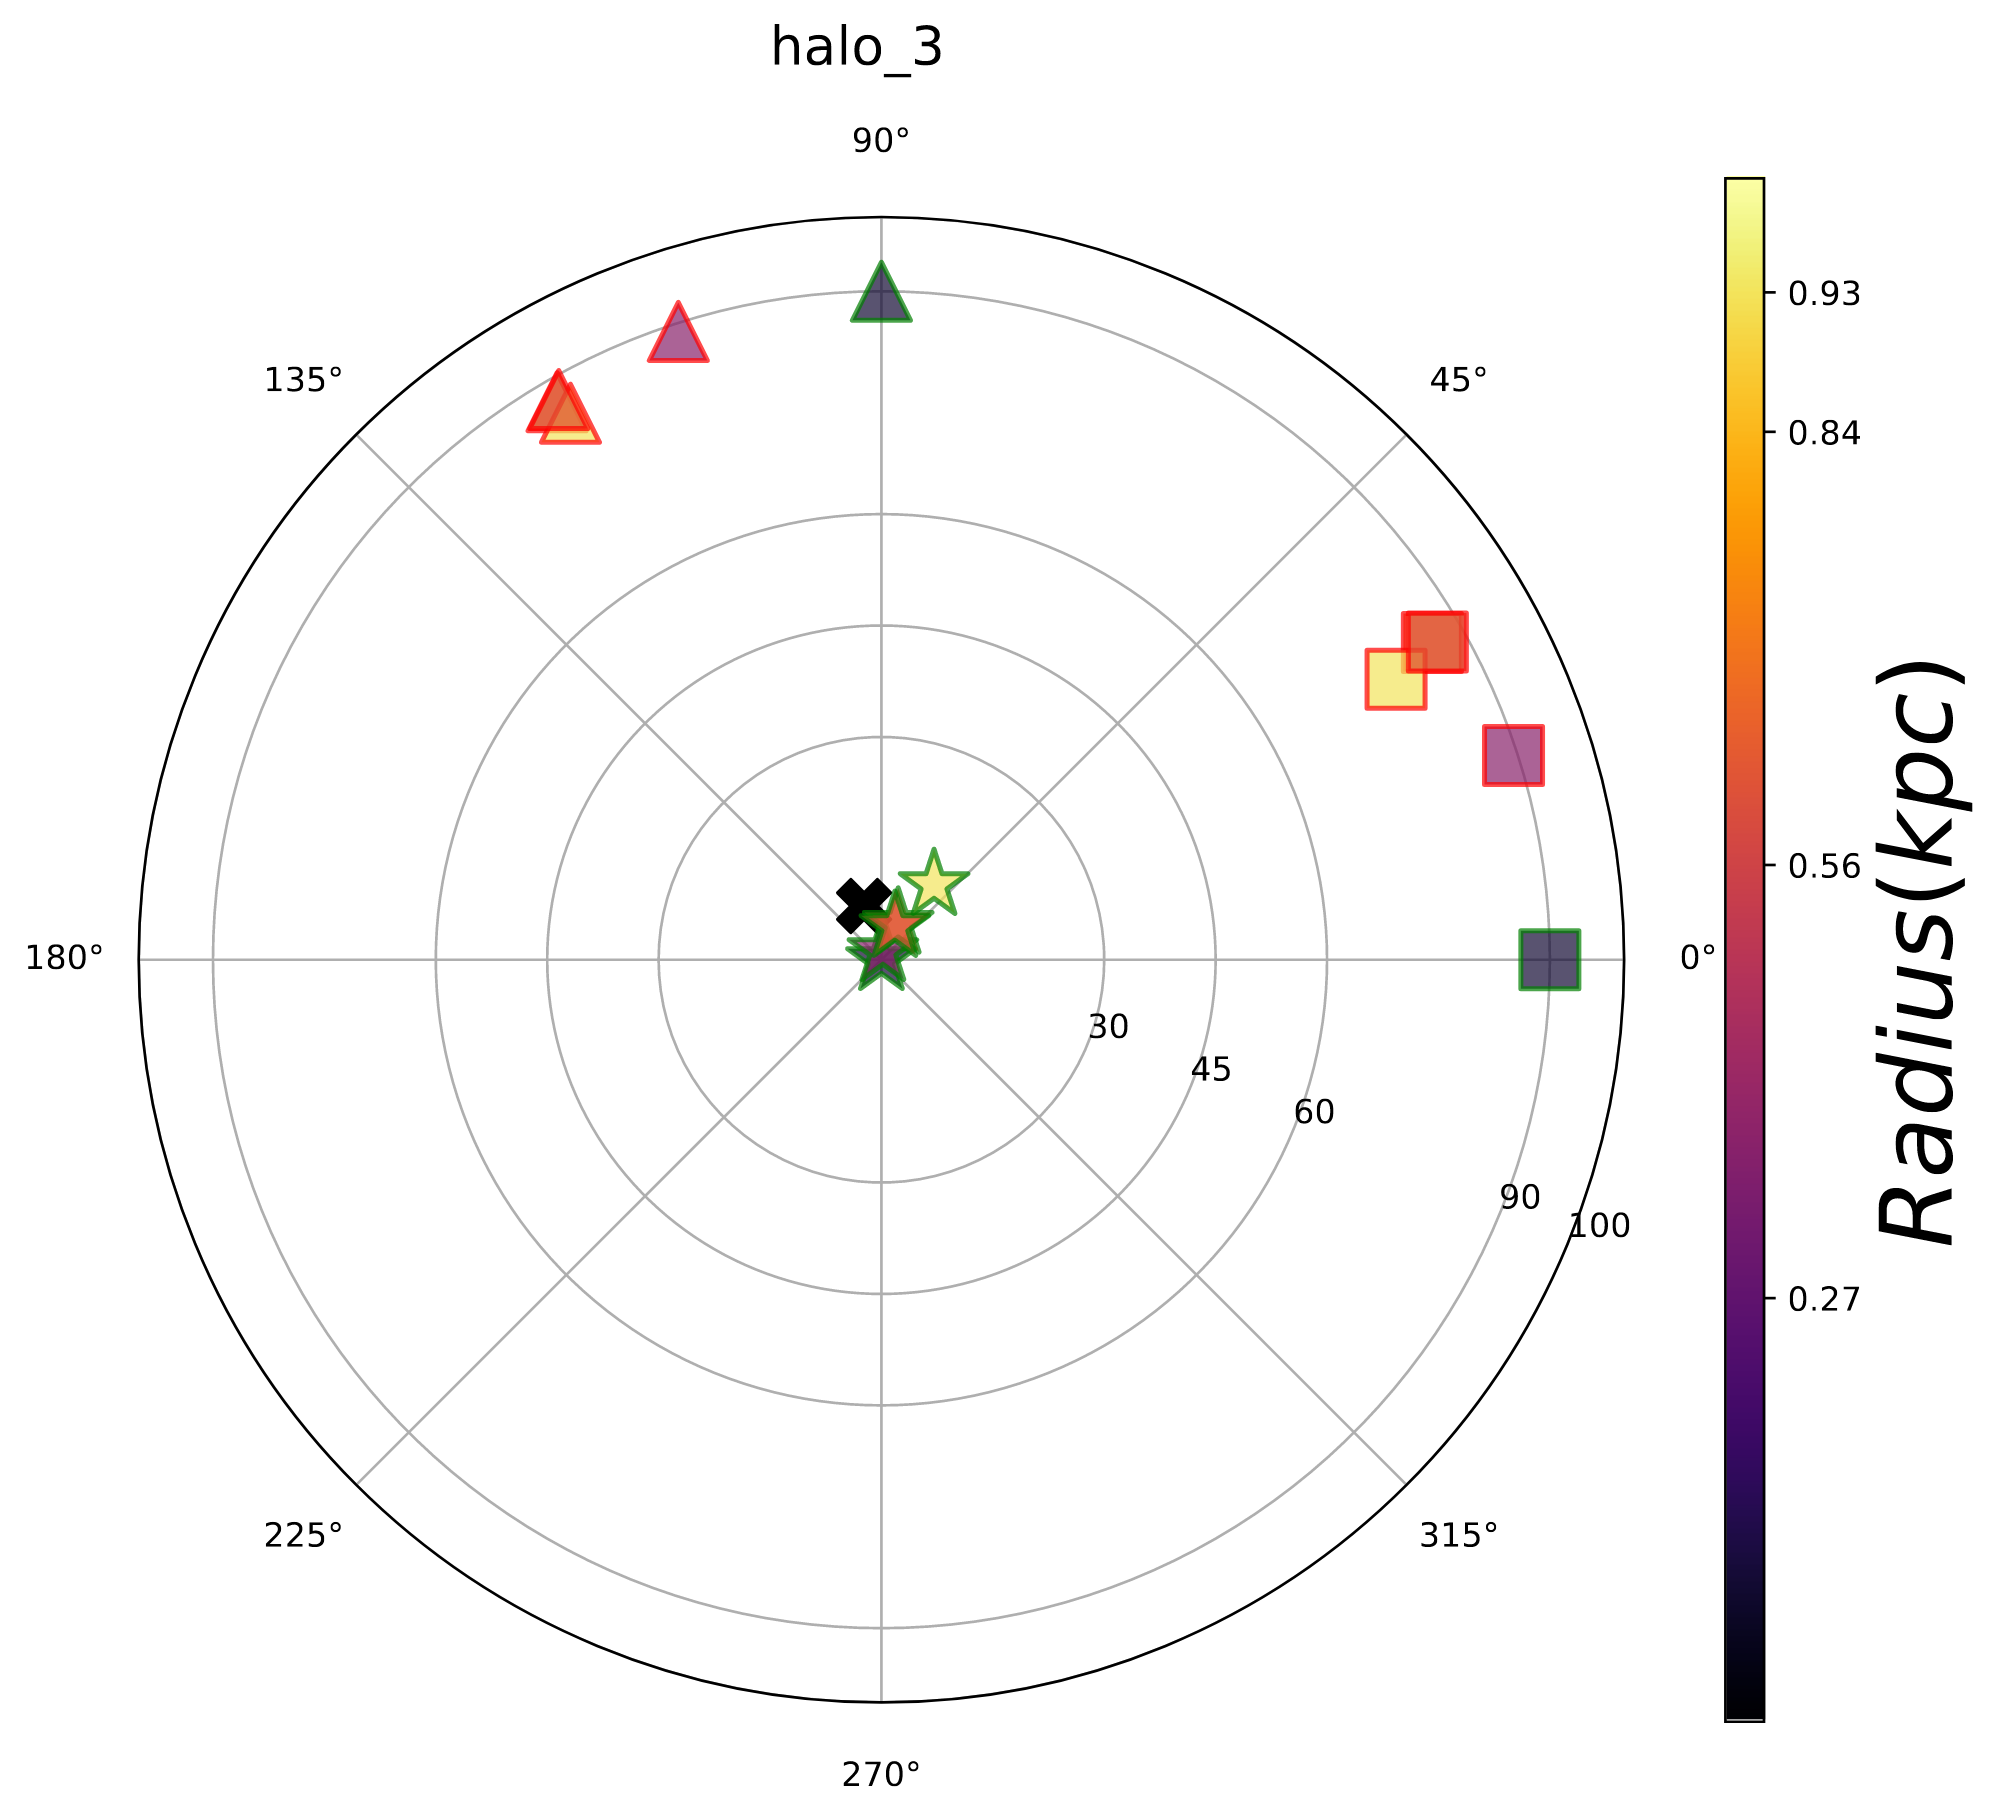
\includegraphics[width=1\columnwidth]{./pics/well_axes.png}}
  \hfill
  \subfloat[Rotating Axes]{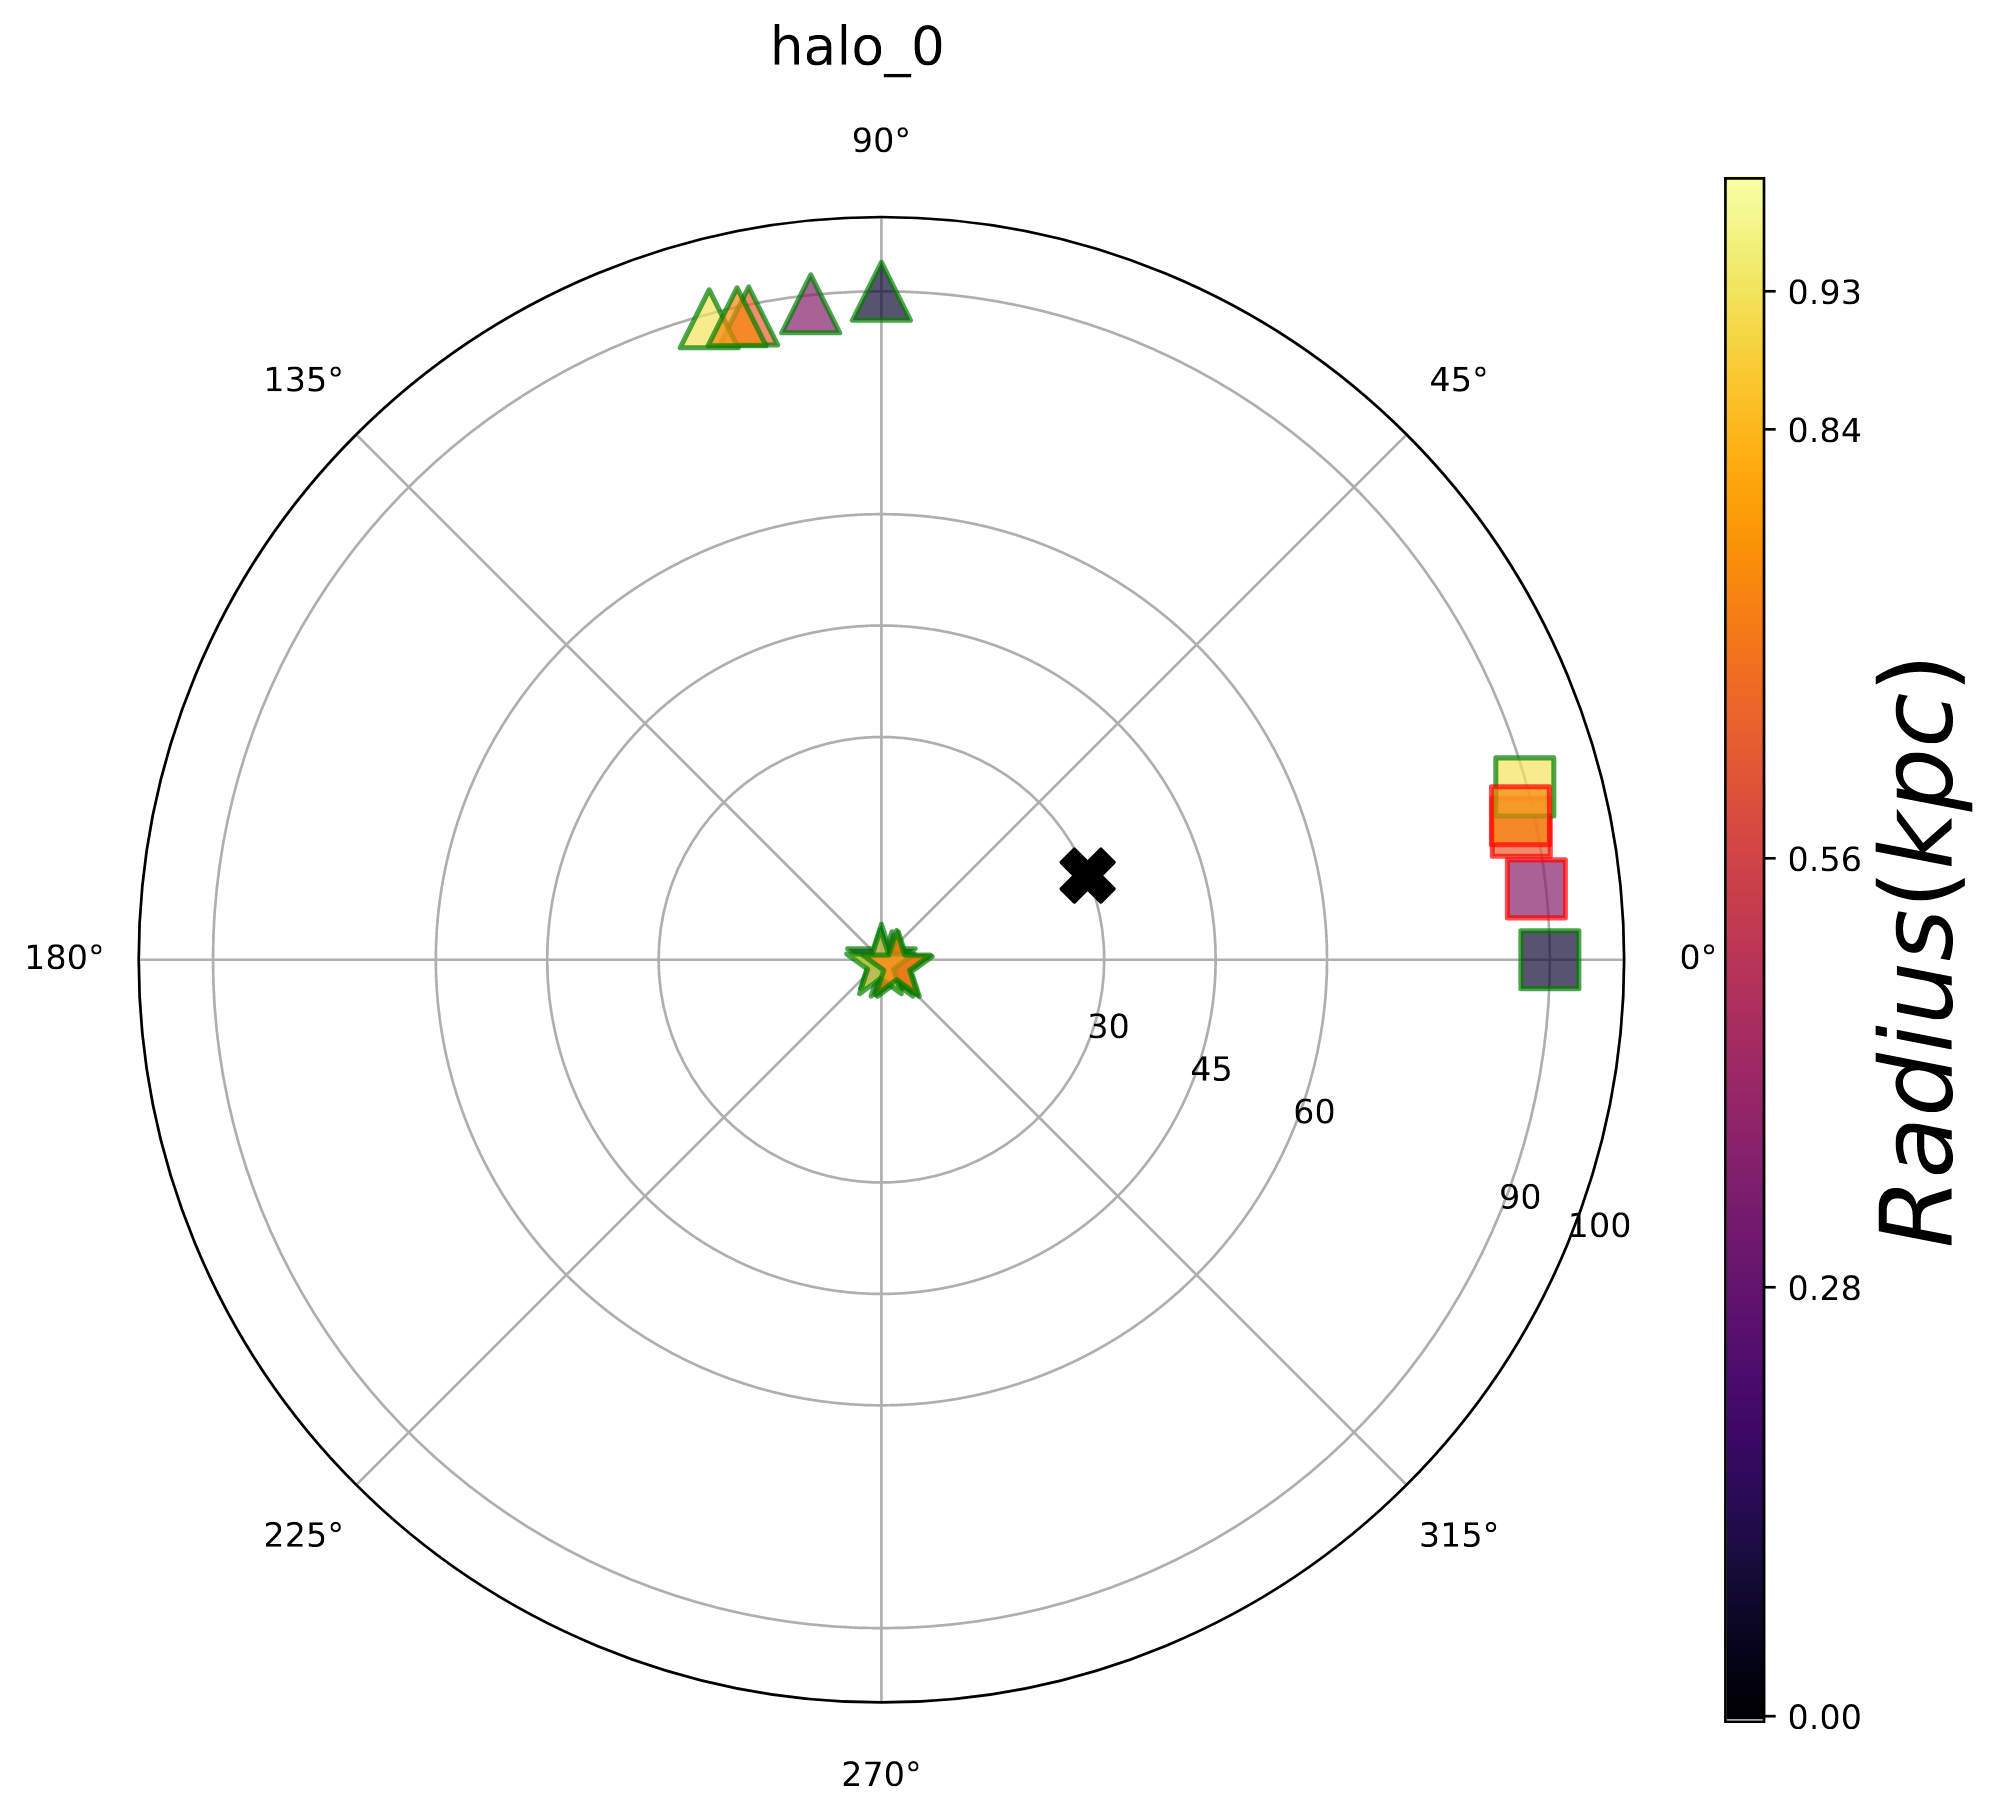
\includegraphics[width=1\columnwidth]{./pics/rotating_axes.png}}
  \hfill
  \subfloat[Chaotic Axes]{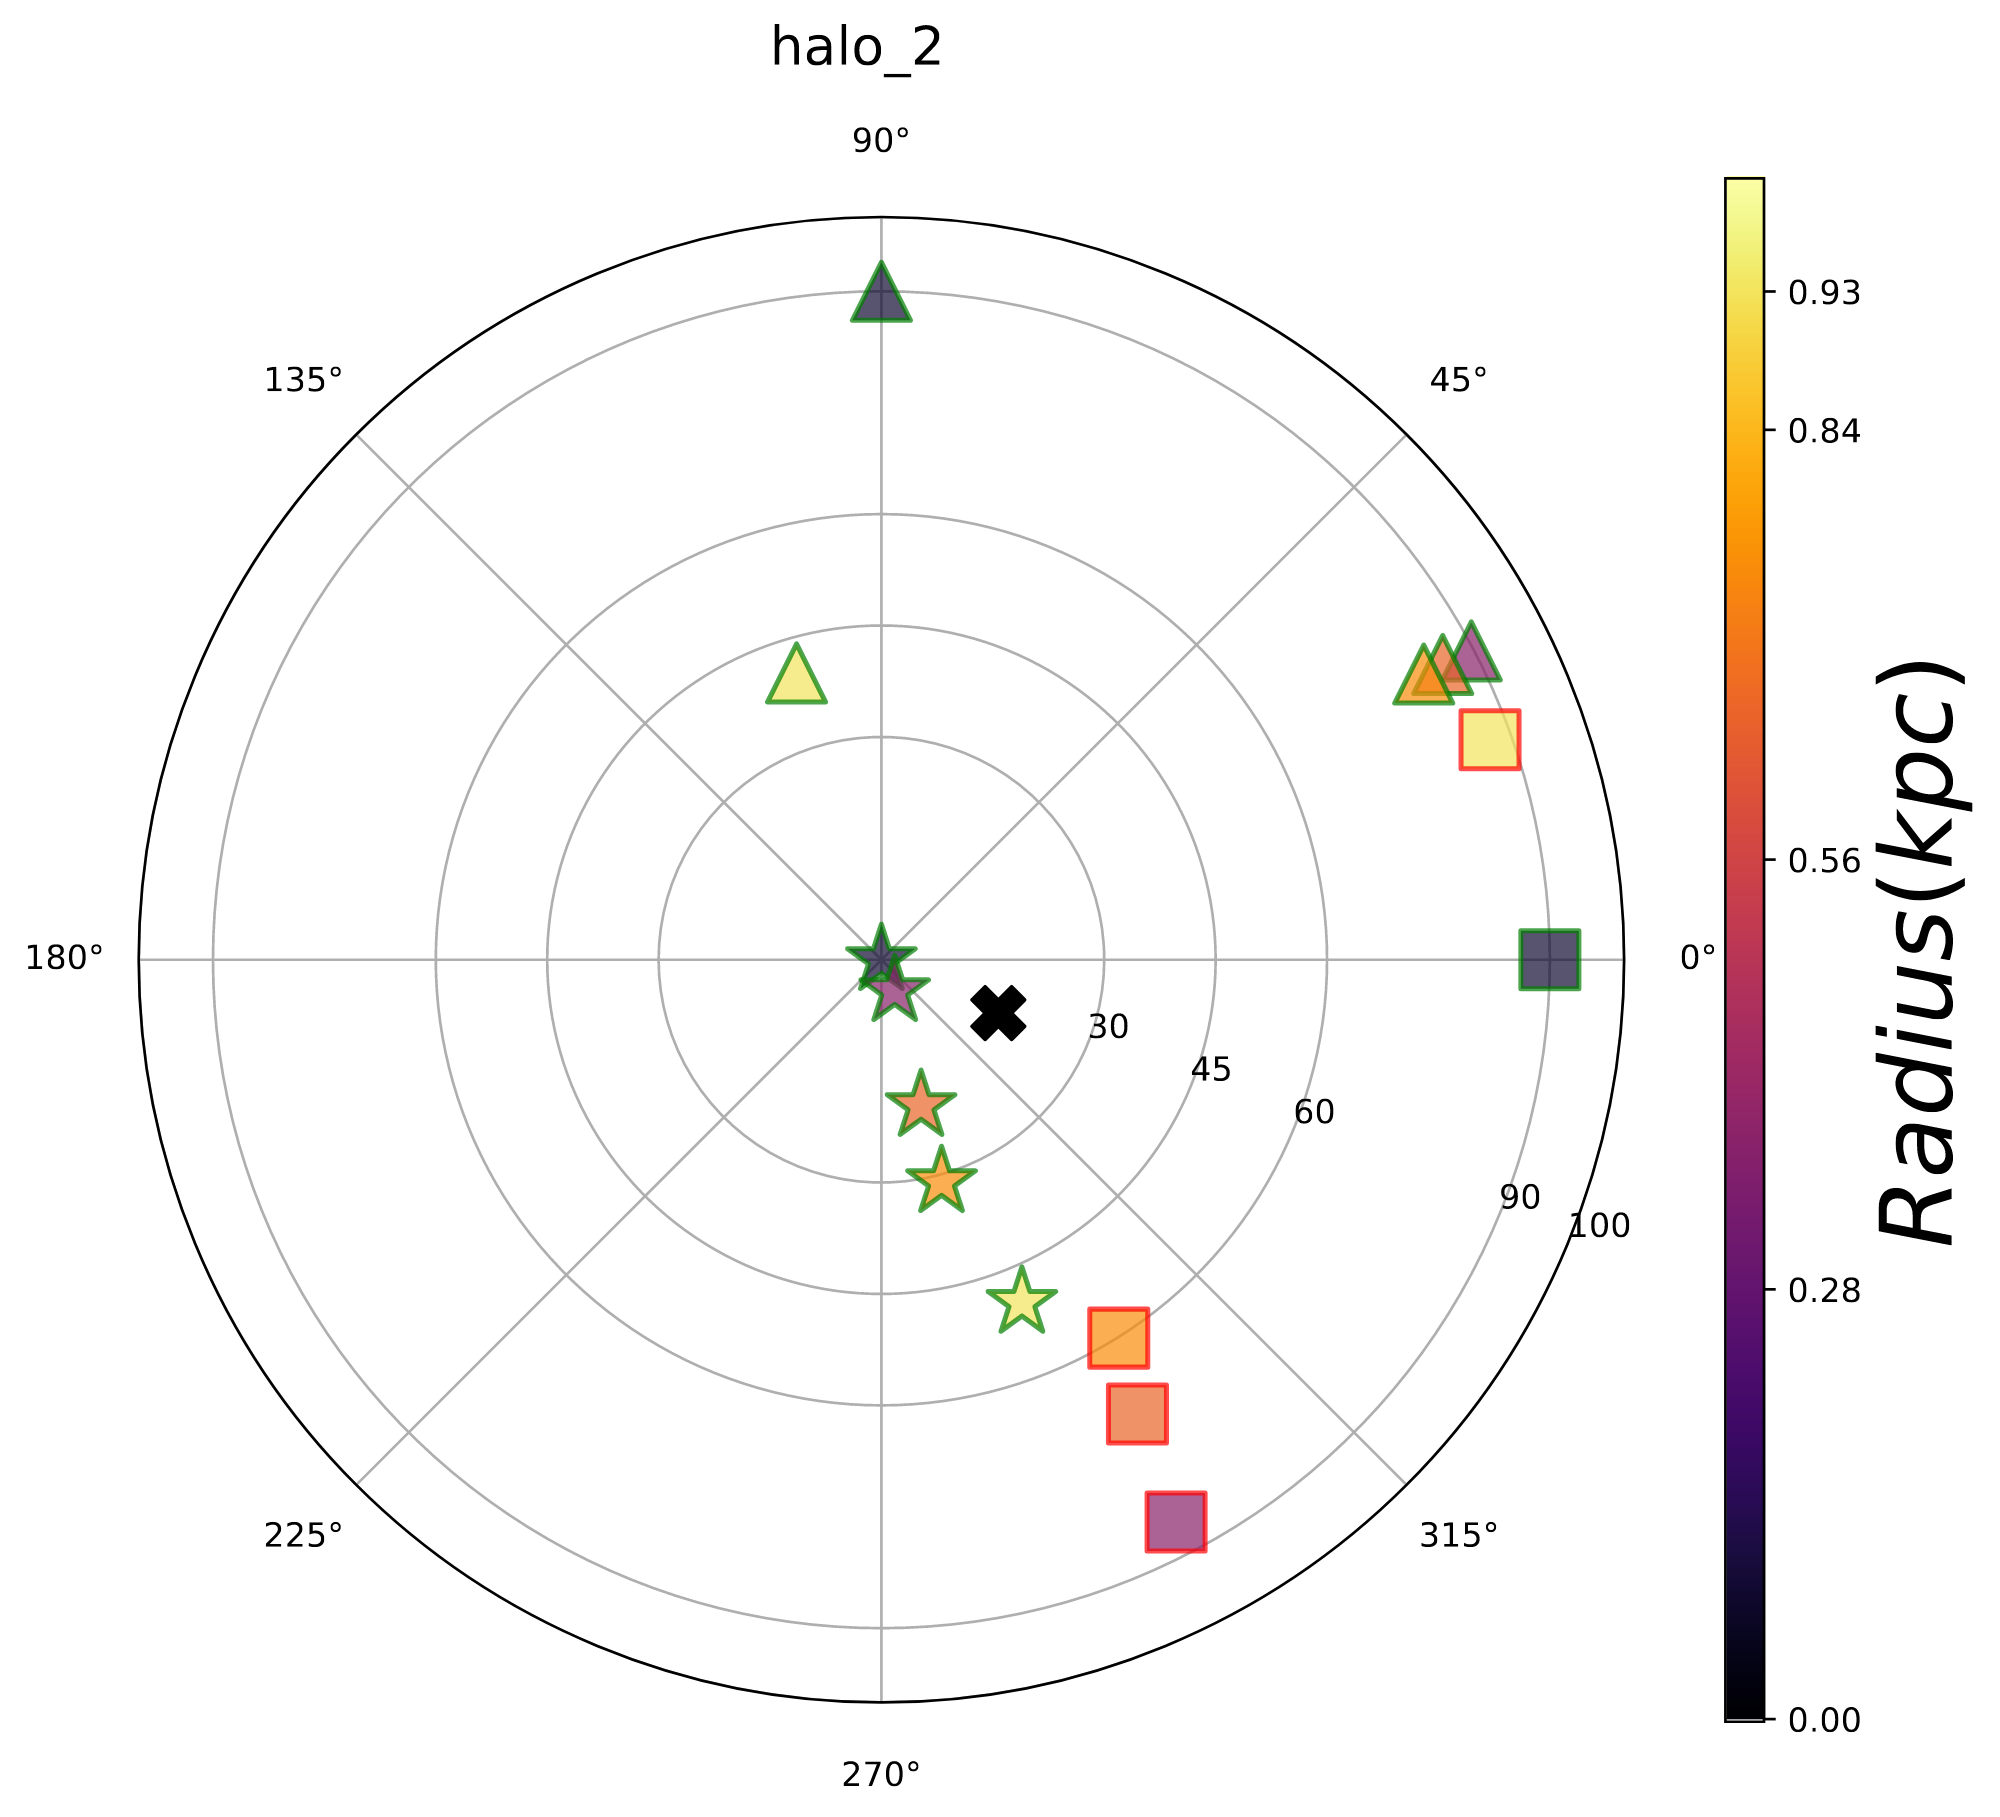
\includegraphics[width=1\columnwidth]{./pics/chaotic_axes.png}}
  \hfill
  \caption{Description of axes alignments }
  \label{fig:slices}
\end{figure}



\section{Conclusions}

The last numbered section should briefly summarise what has been done, and describe
the final conclusions which the authors draw from their work.

\section{Discussion}

\section*{Acknowledgements}



The Acknowledgements section is not numbered. Here you can thank helpful
colleagues, acknowledge funding agencies, telescopes and facilities used etc.
Try to keep it short.

%%%%%%%%%%%%%%%%%%%%%%%%%%%%%%%%%%%%%%%%%%%%%%%%%%

%%%%%%%%%%%%%%%%%%%% REFERENCES %%%%%%%%%%%%%%%%%%

% The best way to enter references is to use BibTeX:

%\bibliographystyle{mnras}
%\bibliography{example} % if your bibtex file is called example.bib


% Alternatively you could enter them by hand, like this:
% This method is tedious and prone to error if you have lots of references
\begin{thebibliography}{99}
\bibitem[\protect\citeauthoryear{Author}{2012}]{Author2012}
Author A.~N., 2013, Journal of Improbable Astronomy, 1, 1
\bibitem[\protect\citeauthoryear{Others}{2013}]{Others2013}
Others S., 2012, Journal of Interesting Stuff, 17, 198
\end{thebibliography}

%%%%%%%%%%%%%%%%%%%%%%%%%%%%%%%%%%%%%%%%%%%%%%%%%%

%%%%%%%%%%%%%%%%% APPENDICES %%%%%%%%%%%%%%%%%%%%%

\appendix

\section{Some extra material}

If you want to present additional material which would interrupt the flow of the main paper,
it can be placed in an Appendix which appears after the list of references.

%%%%%%%%%%%%%%%%%%%%%%%%%%%%%%%%%%%%%%%%%%%%%%%%%%


% Don't change these lines
\bsp	% typesetting comment
\label{lastpage}
\end{document}

% End of mnras_template.tex
